\documentclass{beamer}


% Automaton/graphs package
\usepackage{tikz}
\usetikzlibrary{automata,positioning,arrows.meta,petri}


%Information to be included in the title page:
\usetheme{AnnArbor}
\usecolortheme{beaver}

\title[YAFC]{Projet YAFC}
\subtitle{Yet Another Flight Controller}
\author[OYEZ]{Oussama Felfel \and
Yasmine Benhaddou\texorpdfstring{\\} \and
Elana Courtines \and
Zineb Moubarik}
\institute[UT3]{Université Paul Sabatier}
\date[01/12/2022]{1er Décembre 2022}
\logo{
\includegraphics[height=1cm]{../logoUT3.png}}

\AtBeginSection[]
{
  \begin{frame}
    %\frametitle{Table of Contents}
    \tableofcontents[currentsection]
  \end{frame}
}



\begin{document}

\frame{\titlepage}


\section{Context, Objective}

\begin{frame}
    %\frametitle{Sample frame title}
    Yet Another Flight Controller (YAFC) is a project being held within the Computer Science Master at Université Paul Sabatier.

    \vspace*{5mm}

    Zhenyu Bai expressed their interest in drones. In particular for drones :
    \begin{itemize}
        \item that are cheap to produce ;
        \item physically basic ; 
        \item easily configurable.
    \end{itemize}
    
    \vspace*{5mm}

    The project thus aims to provide a functionnal drone that complies with the aforementioned critierias.
\end{frame}

\begin{frame}
    To function nominally, a drone requires a Flight Controller (FC) to manage the different physical components, as well as some software in order to control how and where it flies. This is what PixHawks, PX4 and ArduPilot provide to name the ones we will be using.

    \vspace*{5mm}

    Unfortunately, today, completely functionnal and ready-to-use drones are expensive. But it is technically possible to produce cheap drones inspired by PixHawks/PX4 or ArduPilot.

\end{frame}

\section{Needs}

\begin{frame}
    
    From a provided functionnal drone frame, Zhenyu Bai expressed the need :
    
    \begin{itemize}
        \item to investigate currently available "almost ready-to-use" options, such as ArduPilot ; 
        \item to make the drone fly using ArduPilot first, then using PixHawks and PX4 ;
    \end{itemize}
    
    \vspace*{5mm}

    Subsequently, gradually, the following objectives will be set :
    
    \begin{itemize}
        \item to produce a custom-made PCB ;
        \item to produce a custom-made Flight Controller inspired by PixHawks and PX4, or possibly by ArduPilot ;
    \end{itemize}
\end{frame}



\section{Organisation}
\subsection{Project Management}
\begin{frame}
    \begin{center}
        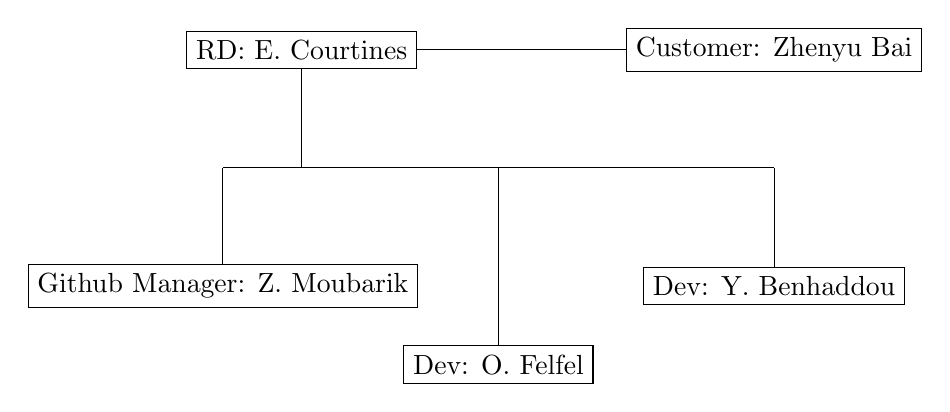
\begin{tikzpicture}
            \node [rectangle,draw] (rd) at (-2.5,0) {RD: E. Courtines};
            \node [rectangle,draw] (client) at (3.5,0) {Customer: Zhenyu Bai};
            \node [rectangle,draw] (l) at (-3.5,-3) {Github Manager: Z. Moubarik};
            \node [rectangle,draw] (m) at (0,-4) {Dev: O. Felfel};
            \node [rectangle,draw] (r) at (3.5,-3) {Dev: Y. Benhaddou};
            \node (link) at (0,-1.5) {};
            \node (aboveleft) at (-3.5,-1.5) {};
            \node (aboveright) at (3.5,-1.5) {};

            \path[-]
            (rd) edge (-2.5,-1.5)
            (link.center) edge (aboveleft.center)
            (link.center) edge (aboveright.center)
            (aboveleft.center) edge (l)
            (aboveright.center) edge (r)
            (link.center) edge (m)
            (rd) edge (client)
            ;

        \end{tikzpicture}
    \end{center}
\end{frame}

\begin{frame}
    \begin{minipage}{0.48\textwidth}
        Project Management Deliverables :
        \begin{itemize}
            \item Kick Off Meeting presentation and minutes (project Plan V0)
            \item Project Plan V1
            \item Project Plan V2
            \item Project Plan V3
            \item "Soutenance"
        \end{itemize}
    \end{minipage}
    \hfill
    \begin{minipage}{0.48\textwidth}
        Technical Deliverables :
        \begin{itemize}
            \item Version 0 : the components work together with ArduPilot ;
            \item Version 1 : the drone can fly with ArduPilot ;
            \item Version 2 : the drone can fly with PX4 and PixHawks ;
            \item Version 3 : the drone can fly with a custom-made PCB and Flight Controller (may be suddivided).
        \end{itemize}
    \end{minipage}
\end{frame}


\subsection{Development Management}
\begin{frame}
    A Github organisation has been created for the project : \href{https://github.com/OYEZ-YAFC}{https://github.com/OYEZ-YAFC}

    \vspace*{10mm}

    A private Repository will contain everything related to the project :
    \begin{itemize}
        \item Arduino programs (C++) ;
        \item Component description files (PCB) ;
        \item Markdown documentation ;
        \item PDFs for the various deliverables, as well as their LaTeX code ;
        \item More depending on how the project evolves.
    \end{itemize}
    
    \vspace*{5mm}

    The Customer will be able to access it.
\end{frame}



\subsection{Customer - Supplier Communication}
\begin{frame}
    Most of the communication will happen on Discord, while the important exchanges will be done by email.

    \vspace*{5mm}

    If needs be, the client will be able to submit issues directly on the Github Repository.
\end{frame}




\end{document}